\chapter{Medicinsk godkendelse}\label{MedicinskGodkendelse}
Den medicinske godkendelse er lavet for at undersøge, hvad der skal til, for at Automatisk Ultralydsscanner kan blive CE-mærket og derved godkendt til markedsføring i Europa. 

Medical Device Directive 93/42/EØF (MDD)\cite{MDD} er hoveddirektivet for medicinsk udstyr i Europa og danner grundlag for de godkendelsesprocedurer, der skal til, for at få medicinsk udstyr CE-mærket. Det er et lovkrav at overholde MDD, når man godkender medicinsk udstyr. MDD er indskrevet i dansk lovgivning ved bekendtgørelse om medicinsk udstyr \cite{Be}.
Alt kursiv i dette afsnit, er citater fra MDD.

\section{Definition}
Medicinsk udstyr er i MDD defineret som: 

\emph{»Medicinsk udstyr«: Ethvert instrument, apparat, udstyr, software, materiale eller anden genstand anvendt alene eller i kombination, herunder software, som af fabrikanten er beregnet til specifik anvendelse til diagnostiske eller terapeutiske formål, og som hører med til korrekt brug heraf, og som af fabrikanten er beregnet til anvendelse på mennesker med
henblik på:}

\let\labelitemi\labelitemii
\emph{\begin{itemize}
\item diagnosticering, forebyggelse, overvågning, behandling eller lindring af sygdomme,
\item diagnosticering, overvågning, behandling, lindring af eller kompensation for skader eller handicap,
\item undersøgelse, udskiftning eller ændring af anatomien eller en fysiologisk proces, eller
\item svangerskabsforebyggelse,
\end{itemize}}

\emph{og hvis forventede hovedvirkning i eller på det menneskelige legeme ikke fremkaldes ad
farmakologisk, immunologisk eller metabolisk vej, men hvis virkning kan understøttes ad denne vej.}

Med udgangspunkt i denne definition af medicinsk udstyr, går Automatisk Ultralydsscanner under kategorien som værende medicinsk udstyr. Dette begrundes med at Automatisk Ultralydsscanners primære opgave er automatiske ultralydsscanninger til srceening for brystkræft, og derved har til formål at forebygge af sygdomme. MDD skal derfor overholdes. 

\section{Klassificering}
Da Automatisk Ultralydsscanner er medicinsk udstyr, skal der foretages en klassificering af systemet. Klassificeringen foretages for at finde ud af hvilken procedure der skal anvendes for at få CE-mærket Automatisk Ultralydsscanner. Klassificeringen afspejler den risiko, der er forbundet med anvendelsen af udstyret. Jo højere klassificering, jo højere risiko er der ved anvendelsen af udstyret og jo længere er godkendelsesproceduren for CE-mærkningen. 

Klassificeringen er som følgende: 

\let\labelitemi\labelitemii
\begin{itemize}
\item Klasse I - Udstyr med lav risiko for beskadigelse af bruger/patient. Inføres ofte ikke i kroppen.
\item Klasse IIa - Udstyr med reduceret risiko for beskadigelse af bruger/patient. Bruges kort tid og tilføres energi eller indføres i kroppen.  
\item Klasse IIb -  Udstyr med risiko med beskadigelse af bruger/patient. Bruges i længere tid og tilføres energi eller skal indføres i kroppen. 
\item Klasse III - Udstyr med høj risiko for beskadigelse af bruger/patient i tilfælde af fejl. F.eks hjerteklapper. 
\end{itemize} \cite{Delta}

I MDD, er der 18 regler, man klassificerer medicinsk udstyr ud fra. 

Regel 10 omhandler aktive anordninger beregnet til diagnosticering og overvågning af vitale fysiologiske processer. Dette passer på Automatisk Ultralydsscanner, da det er et system, som er tilsluttet en ultralydsscanner, hvilket gør Automatisk Ultralydsscanner til en aktiv anordning.  

Citat fra MDD regel 10. 
\emph{Aktiv anordninger, der er beregner til diagnosticering, henhører under klasse IIa: - hvis de er beregnet til at muliggøre en direkte diagnosticering eller overvågning af vitale fysiologiske processer...}

Da Automatisk Ultralydsscanner er beregnet til overvågning af vitale fysiologiske processer og ikke skal bruges på patienter i længere tid, er Automatisk Ultralydsscanner klasse IIa. 

\section{CE-Mærkning}
Klassificering af Automatisk Ultralydsscanner danner grundlag for proceduren for CE-mærkning. 

Inden Automatisk Ultralydsscanner kan CE-mærkes, skal producenten igennem en række godkendelsesprocedurer. Definering og klassificering, som er gjort overfor, er en del af de procedure, producenten skal udføre. Derudover skal producenten overholde væsentlige krav fra MDD. Der skal udarbejdes teknisk dokumentation for produktet, bestående af en risikoanalyse og klinisk evaluering. Producenten skal ydermere lave et kvalitetssikringssystem og have et post market surveillance system, et system for hvordan producenten vil holde øje med produktet og andre lignende produkter, når det er kommet ud på markedet. Derudover skal producenten have en EF-overensstemmelseserklæring, hvor der  erklæres at produktet opfylder bekendtgørelsens krav \cite{Vej}. Når EF-overensstemmelseserklæring er underskrevet, kan producenten påføre CE-mærket. Som producent i Danmark, skal man registreres hos Lægemiddelstyrelsen, før markedsføringen kan påbegyndes. Producenten kan selv vælge et bemyndiget organ, som godkender, at producentens dokumentation lever op til gældende lovgivning. \cite{Klasse} 

Godkendelsesproceduren er et stort arbejde, da MDD er kompliceret at læse og forstå. Godkendelsesproceduren kan gøres lettere ved i stedet at følge en række standarder, som er harmoniseret i forhold til MDD. Til den medicinske godkendelse af Automatisk Ultralydsscanner er de harmoniserede standarder til risikohåndteringen DS/EN ISO 14971:2012 \cite{14971} og kvalitetssikring DS/EN ISO 13485:2012 \cite{13485} blevet anvendt. Se hvordan standarterne er anvendt nedenfor. 

\subsection{Risikohåndtering}
Da projektet er et undersøgelsesprojekt og udviklet for at teste muligheden for at udføre automatiserede ultralydsscanninger til screening for brystkræft. Og at udviklingsforløbet startede før der var kendskab til kravet om en risikohåndtering, er Automatisk Ultralydsscanner ikke udviklet med hensyn til risikohåndteringen. Der er dog stadig udført risikohåndtering på Automatisk Ultralydsscanner, hvor DS/EN ISO 14971:2012 \cite{14971} er blevet fuldt, for at vurdere risikoniveuet for Automatisk Ultralydsscanner som et færdigt produkt. 

I risikoanalysen, blev der identificeret risici ved Automatisk Ultralydsscanner. De identificerede risici blev vurderet ved at se på sandsynlighed for at risicien ville opstå samt en konsekvens af at risicien opstod. Sandsynligheden blev vægtet fra 1-5, hvor 1 var meget usandsynlig og 5 var meget sandsynlig. Konsekvensen blev også vurderet fra 1-5, hvor 1 var ubetydelig og 5 var ødelæggende. Hver risici blev vurderet med en kombination af sandsynlighed og konsekvens. Se bilag \ref{Godkendelsesprocedure} Godkendelsesprocedure, for at se hvordan risici er identificeret samt hvordan risiciene er blevet analyseret. 

I risikoevalueringen blev risiciene indtaget i en risikomatrix, som tydeliggør kombinationen af sandsynligheden og konsekvensen. Risikomatrixen gør det let at overskue, hvilke risici som skal reduceres samt det samlede risikoniveau for Automatisk Ultralydsscanners.  

Tabel \ref{Niveau} viser risikomatrixens farvers betydning. 

\begin{figure}[H]
    \centering
    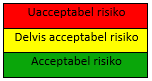
\includegraphics[width=0.30\textwidth]{figurer/r/Niveau}
    \caption{Risikomatrixens farvers betydning}
    \label{Niveau}
\end{figure}

Tabel \ref{Risiko} viser de fundne risici for Automatisk Ultralydsscanners samlet i en risikomatrix. Tallene i risikomatrixen henviser til de fundne risici fra risikoanalysen, se bilag \citep{Godkendelsesprocedure} Godkendelsesprocedure, afsnit om risikoanalyse.  

\begin{figure}[H]
    \centering
    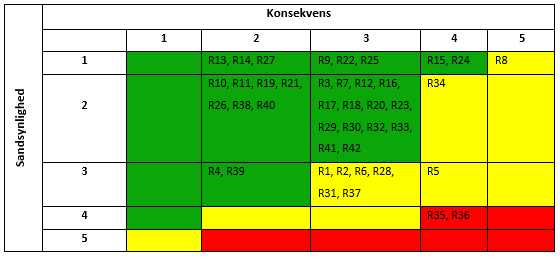
\includegraphics[width=1\textwidth]{figurer/r/Risiko}
    \caption{Risikomatrix}
    \label{Risiko}
\end{figure}

ISO 14971:2012 specificerer ikke hvad en acceptabel risiko er, men producenten er altid forpligtiget til at reducere risici mest muligt \cite{14971}. Ud fra risikomatrixen ligger Automatisk Ultralydsscanners samlede risikoniveau, i den acceptable ende, da der er flest risici i det grønne område. Risiko R35 – \textit{Kalibrering mellem robotarm og 3D kamera er forkert} og R36 - \textit{Bevægelsesmønster af robotarm er uhensigtsmæssigt}, ligger i det uacceptable niveau. Derfor bør der laves risikoreduktion på disse to risici, hvor muligheden for at mindske sandsynligheden for at risiciene vil opstå vurderes. Dette kunne f. eks ske ved at lave hyppige tests af systemet, oplæring af Operatør i hvordan Automatisk Ultralydsscanner kalibreres, samt en detaljeret beskrivelse af hvad et hensigtsmæssigt bevægelsesmønster, for Automatisk Ultralydsscanner, er. Se bilag \ref{Godkendelsesprocedure} Godkendelsesprocedure, afsnit om Risikohåndtering for at se hvordan risikohåndteringen er foretaget. 

\subsection{kvalitetssikring}
Når man producere medicinsk udstyr, skal man også have et Kvalitetsstyringssystem (QMS). QMS dækker over en dokumenteret plan for, hvordan producenten sikrer at opfylde kravene specificeret i lovgivningen og kan opfyldes ved at følge ISO 13485:2012 \cite{13485}. Et QMS skal indeholde oplysninger om organisationen, ansvarsfordeling, arbejdsprocesser og procedure samt ressourcer der er til rådighed i produktionen. Derudover skal der være sporbarhed i alle dokumenter og komponenter der er anvendt i produktet, så man kan finde tilbage i produktet ved eventuelle fejl. \cite{13485}
Der er ikke udviklet et kvalitetssikringssytem over Automatisk Ultralydsscanner. Se bilag \ref {Godkendelsesprocedure} Godkendelsesprocedure, afsnit om Kvalitetssikring, hvor det beskrives hvordan et kvalitetssikringssystem kan udvikles. 

\section{Softwaregodkendelse}
Da Automatisk Ultralydsscanner har software, som styrer robotarmen, skal krav til medicinsk software også overholdes. Der er krav om en dokumenteret udviklingsproces, vedligeholdelsesplan, risikohåndtering og plan for løsning af softwarefejl. Standarden DS/EN 63204:2006 - Software for medicinsk udstyr - Livscyklusprocesser for software \cite{software} er anvendt, til at beskrive hvordan krav til medicinsk software kan overholdes. Se bilag \ref {Godkendelsesprocedure} Godkendelsesprocedure, afsnit om Softwaregodkendelse.

Den fulde medicinske godkendelse kan ses i bilag \ref {Godkendelsesprocedure} Godkendelsesprocedure.
